% 1964 全国卷第 8 题：面积和最小时两圆等半径（矢量重绘）
\begin{tikzpicture}[scale=0.8]
  \draw (0,0) rectangle (4,4);
  \draw (1.172,1.172) circle (1.172);
  \draw (2.828,2.828) circle (1.172);
  \fill (1.172,1.172) circle (1.2pt) node[below left] {$O$};
  \fill (2.828,2.828) circle (1.2pt) node[above right] {$O'$};
  \node at (2,-0.72) {$r=r'=\dfrac{2-\sqrt2}{2}$};
\end{tikzpicture}
